%\documentclass{acm_proc_article-sp}
\documentclass{sig-alternate}
\usepackage{amsmath}
\usepackage{amssymb}
\usepackage{listings}
\usepackage{courier}
\usepackage{multirow}

% Include PDF graphics, configure our images directory, and specify image types.
\usepackage{graphicx}
\usepackage{epsfig}
\graphicspath{{./images/}}
\DeclareGraphicsExtensions{.pdf,.jpeg,.png,.jpg}

% Style listings
\lstset{%rulesepcolor=\color{Gray},
        frame=single,                        	% Shadow box frame around code
        basicstyle=\scriptsize\ttfamily,        % Use small true type font
        showstringspaces=false,                 % Don't put marks in string spaces
        morecomment=[l][\color{Blue}]{...},     % Line continuation (...) like blue comment
}

\begin{document}

\title{Toward Quantitative Emulation of Cloud Robotic Systems}

\numberofauthors{1}

\author{
\alignauthor
Christopher C. Lamb, Rafael Figueroa, Rafael Fierro\\
       \affaddr{University of New Mexico}\\
       \affaddr{Department of Electrical and Computer Engineering}\\
       \affaddr{Albuquerque, NM 87131-0001}\\
       \email{\{cclamb, rafa, rfierro\}@unm.edu}
}

\conferenceinfo{ICCPS '14,} {April 14-17, 2014, Berlin, Germany.} 
\CopyrightYear{2014} 
\crdata{978-1-4503-1005-5/11/10} 
\clubpenalty=10000 
\widowpenalty=10000

\maketitle

\begin{abstract}
Insert abstract here.
\end{abstract}

\category{D.2.11}{Software}{Software Architectures}[Domain-specific Architectures]
\terms{Design, Performance, Robotics}
\keywords{Robotics, Cloud}

\section{Introduction}
Introduction to topic; why it is important, motivate reader.

\section{Cyber-physical Clouds}
Highlight the problem we are starting to address.

\subsection{A Taxonomy of Architectures}
Outline an initial taxonomy.

\subsection{Initial Analysis of Taxonomy}
Notionally analyze the taxonomy.

\subsection{Future Work}
Where to next.

\section{Related Work}
Cover previous work in area, especially motivating work.

\section{Summary and Conclusions}

%\begin{figure}[!t]
%\centering
%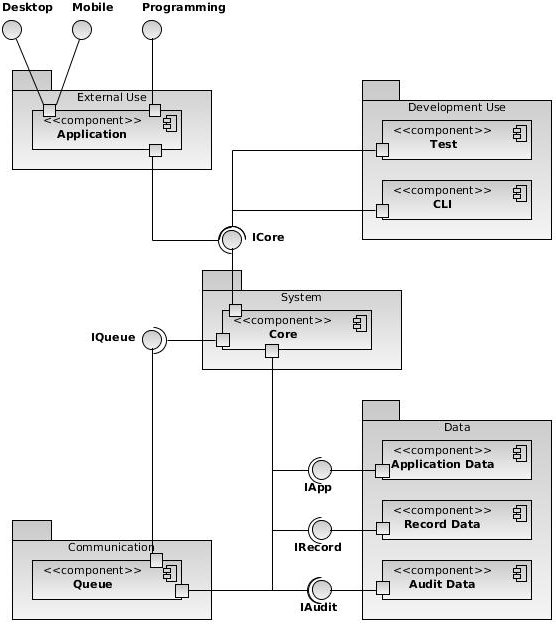
\includegraphics[width=3in]{HisbSystemArch}
%\caption{System Architecture Runtime Component View}
%\label{fig:RuntimeView}
%\end{figure}

\bibliographystyle{abbrv}
\bibliography{bib/cps.bib}

\end{document}


